\documentclass{article}

% Define margins
\setlength{\topmargin}{-1.0cm}
\setlength{\oddsidemargin}{0.1cm}
\setlength{\textwidth}{16.5cm}
\setlength{\textheight}{23.0cm}

\usepackage{graphicx} %LaTeX package to import graphics
\graphicspath{{images/}} %configuring the graphicx package

% Define header and footer
\usepackage{fancyhdr}
\pagestyle{fancy}
\fancyhf{}
\lhead{{
\includegraphics[height=.65cm]{buetlogo.png}}}
\rhead{\textbf{\textit{Snort3}} }
\cfoot{\textbf{\textit{\thepage}}}
\renewcommand{\headrulewidth}{0.7pt}
\setlength{\headheight}{23pt}
% This is to define a style with no footer for the table of contents
\fancypagestyle{nofooter}{%
  \fancyfoot{}%
}

% To manage references
\usepackage{natbib}

\begin{document}

\begin{center}
\vspace{1.5cm}


\includegraphics[width=0.4\textwidth]{images/buetlogo.png}\\
\vspace{0.3cm}
\vfill

{\LARGE \textbf{ Final Project of CSE406 (Computer Security Sessional)}}

\vspace*{3\baselineskip}

{\LARGE \textbf{Project : Snort 3}}\\
{\LARGE \textbf{Tool : NIDS}}
\begin{large}
\vspace*{2\baselineskip}

Submission Date: \today

\vspace*{2\baselineskip}

\emph{submitted by} \\[1.5ex]
{\Large \textbf{1905048 (Al-Amin Sany)} \\ \par} 
% \vspace{0.5cm}
{\Large \textbf{1905052 (Bijoy Ahmed Saiem)} \\ \par} 

\vspace{1.5cm} \\

Under the supervision of \\ % Tagline(s) or further description
[\baselineskip] % Tagline(s) or further description
\textbf{Abdur Rashid Tushar}\\
Lecturer\\
{Computer Science and Engineering Department}\\
{Bangladesh University of Engineering and Technology}\\

\thispagestyle{empty} 

\end{large}
\end{center}
\pagebreak

% \lhead{\emph{Contents}} % Set the left side page header to "Contents"
\tableofcontents
	\thispagestyle{nofooter}
	\cleardoublepage
	\typeout{}

\pagebreak

\setcounter{page}{1}

\section{Abstract}
\label{sec:Abstract}
\begin{center}

\includegraphics[width=0.4\textwidth]{images/snort3_logo.png}  
\end{center}
\fontsize{18pt}{25pt}\selectfont Snort, created by Martin Roesch in 1998, is a versatile IDS/IPS that offers real-time analysis of network traffic to detect and respond to potentially malicious activities. It operates on a rule-based system, where users can define custom rules or employ pre-existing rule sets to identify and mitigate threats. Snort’s rule-based approach allows it to monitor network traffic at both the network and application layers, thereby offering comprehensive protection against a wide range of network-based attacks and vulnerabilities. Snort represents a vital asset in the arsenal of network security tools. Its rule-based detection, adaptability, and open-source philosophy have established it as a trusted solution for identifying and mitigating network threats. As cyber threats continue to evolve, Snort’s role in defending against these threats remains indispensable, ensuring the resilience of modern network infrastructures. \\\\
\clearpage

\section{Introduction}
\label{sec:Introduction}

\subsection{What is Snort3}
 Snort is a popular free and open-source IDS/ IPS system that is used to perform traffic/
 protocol analysis and content matching. Snort can be used to detect and prevent various
 attacks based on predefined rules.
 
\subsection{ Snort Operations}
\begin{itemize}
  \item \textbf{Packet Sniffing:} Analyzes the actual network traffic in real-time
  \item  \textbf{Network Intrusion Detection and Prevention:} Analyzes packets and matches traffic against signatures and drop packets.
  \item \textbf{Packet Logging:} Collects and logs network traffic into a log file
\end{itemize}

\subsection{How Does Snort3 Work?}
 Snort detects malicious traffic or attacks by leveraging pattern matching. When active,
 Snort captures packets, reassembles them, analyzes them, and determines what needs
 to be done to the packet based on predefined rules.
 Snort has a large number of rule sets created by the community that are very useful
 to begin with. Snort rules are very similar to a typical firewall rule, whereby, they are
 used to match network activity against specific patterns or signatures and consequently
 make a decision as to whether to send an alert or drop the traffic (in the case of IPS).

 \subsection{Snort3 Rules}
 \begin{itemize}
  \item \textbf{Community Rules:} Free rule sets created by the Snort community.
  \item  \textbf{Registered Rules:} Free rule sets created by Talos. In order to use them, a user must register for an account.
  \item \textbf{Subscription Only Rules:} These rule sets require an active paid subscription
 in order to be accessed and used.
  \item \textbf{Customized Rules:} We can write our own rules based on our requirements.
\end{itemize}
The syntax of customized rules are: \\\\
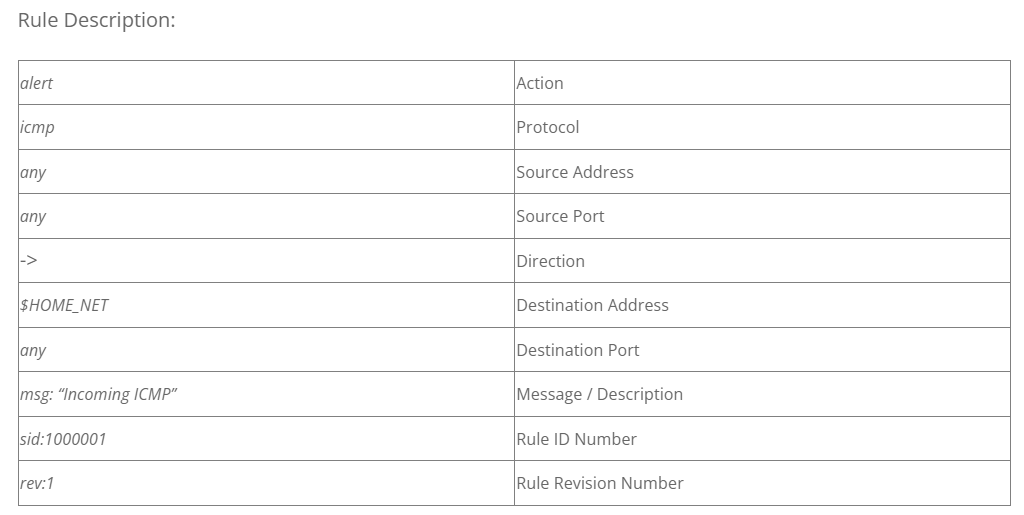
\includegraphics[width=1.0\textwidth]{images/snort_rule.png} 
\clearpage

\section{Prerequisites}
\label{sec:Task3}
\subsection{Virtual Machine Setup}
Four VMs are used for this project:\\\\
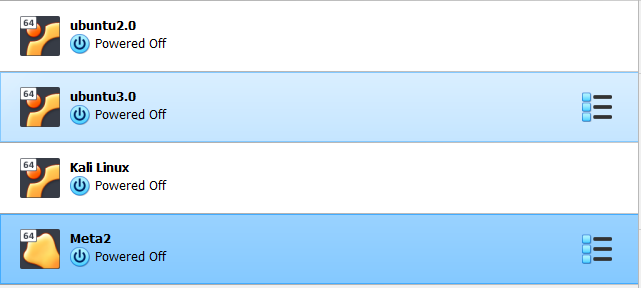
\includegraphics[width=1.0\textwidth]{images/vms_list.PNG}\\\\
The roles of these VMs are:
\begin{itemize}
 \item \textbf{ubuntu2.0:} Snort3 is installed here.
 \item \textbf{ubuntu3.0:} Vulnerable Machine.
 \item \textbf{kali linux:} Attacker Machine
 \item \textbf{Meta2:} More vulnerable Machine.
\end{itemize}
\clearpage
\hspace{-\3.5cm}The IP addresses of all Virtual Machines must be within the same subnet to connect with each other.\\\\
IP addresses of the four VMs:\\
\begin{itemize}
 \item \textbf{ubuntu2.0:} 192.168.48.4
 \item \textbf{ubuntu3.0:} 192.168.48.5
 \item \textbf{kali linux:} 192.168.48.6
 \item \textbf{Meta2:} 192.168.48.7
\end{itemize}
\vspace{3cm}
\subsection{Snort3 Installation}
\textbf{We follow this link to install snort3:}\\
\href{https://cytoolz.com/blog/snort-3-install-and-configure-intrusion-detection-system-on-ubuntu-22-04}\\\\
\textbf{Youtube Link:}\\
\href{https://youtu.be/uPdCmuFh40M?si=gJXhh7eJ9ibMkw4R}
\clearpage

\section{Demonstration}
\label{sec:Demonstration}
\subsection{Pakcet Sniffing}
 Packet sniffing in Snort refers to the capability of the Snort Intrusion Detection System (IDS) to capture and inspect network packets as they traverse a network interface. It is one of the fundamental functions of Snort, allowing it to analyze network traffic in real-time for the detection of suspicious or malicious activity. Packet sniffing specifically refers to the process of capturing and inspecting network packets as they traverse a network interface. This is the initial step where the IDS monitors the raw network traffic for any suspicious or malicious activity. So, we are not demonstrating this feature separately and we are jumping to Intrusion Detection directly.
\subsection{Network Intrution Detection}
Snort3 rules operate similarly to conventional firewall rules. They are designed to analyze network activity, looking for specific patterns or signatures. When a match is found, Snort3 can take action by either generating an alert or dropping the packet if configured as an Intrusion Prevention System (IPS). This proactive approach helps in enhancing network security by identifying and responding to potential threats in real-time. For verifying this a home network is created below.
\clearpage
\begin{itemize}
\item \textbf{A Home Network(Name : snortyNet , IP : 192.168.48.0/24) is Created:}\\\\
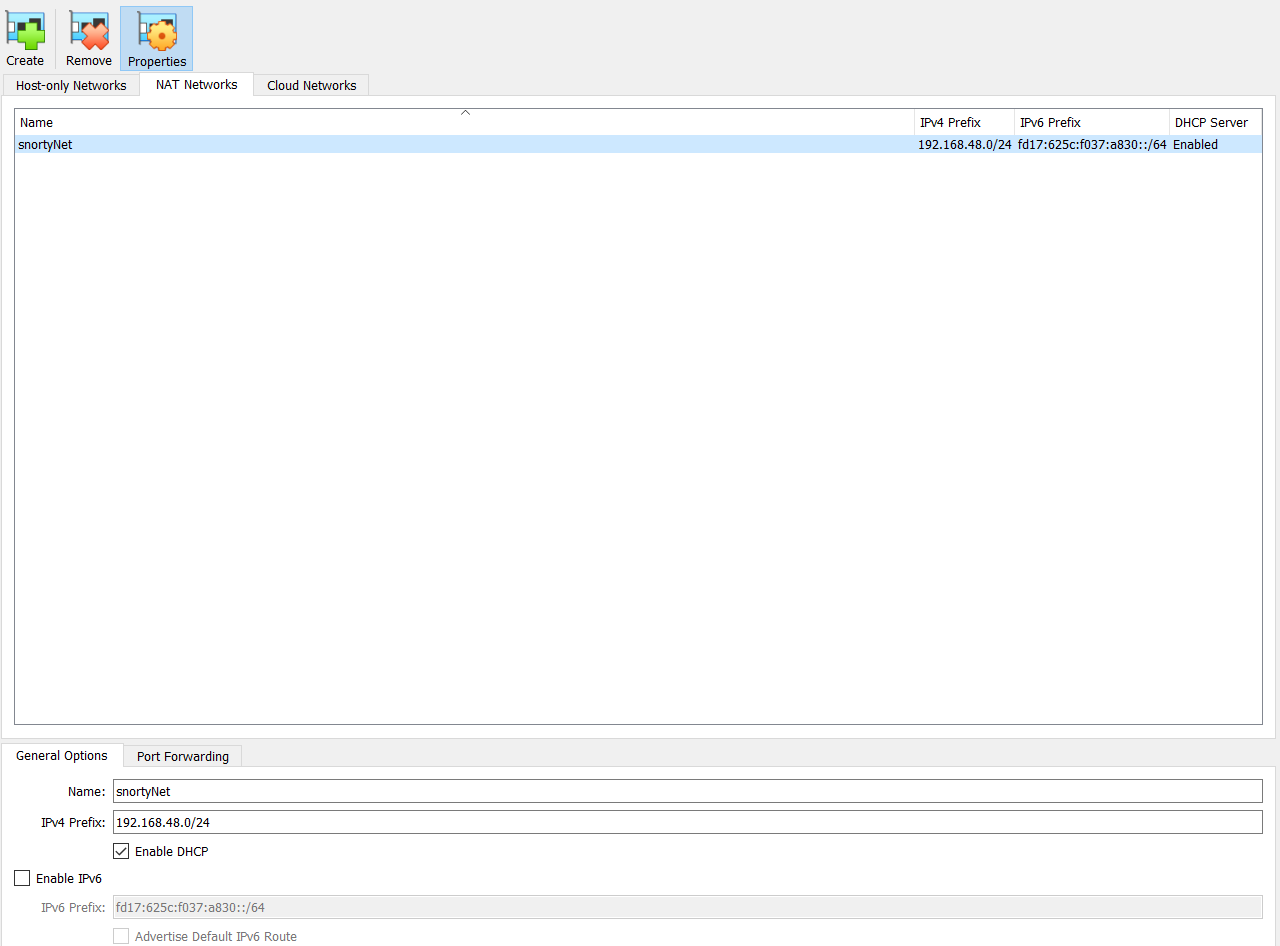
\includegraphics[width=1.0\textwidth]{images/network_creation.PNG}
\end{itemize}
\clearpage
\begin{itemize}
    \item \textbf{Virtual Machines are connected to the Home Network:}\\\\
    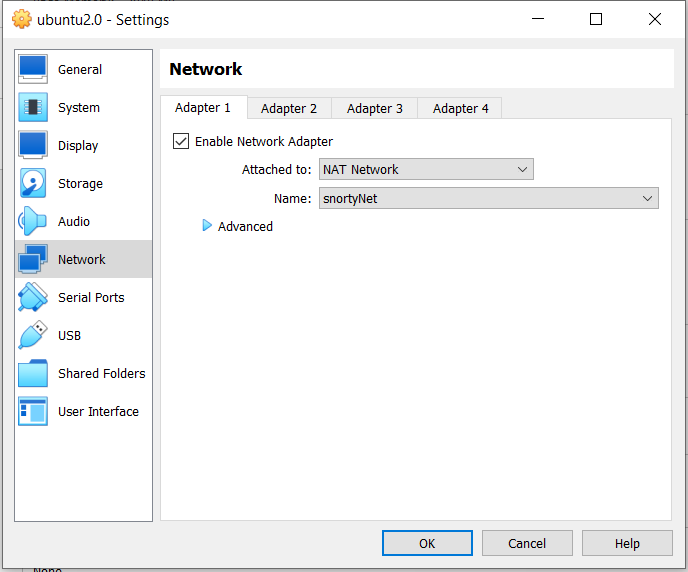
\includegraphics[width=1.0\textwidth]{images/device_connection.PNG}
\end{itemize}
\clearpage
\begin{itemize}
    \item \textbf{The IP addresses of all Virtual Machines are set within the same subnet to connect with each other.}\\\\
    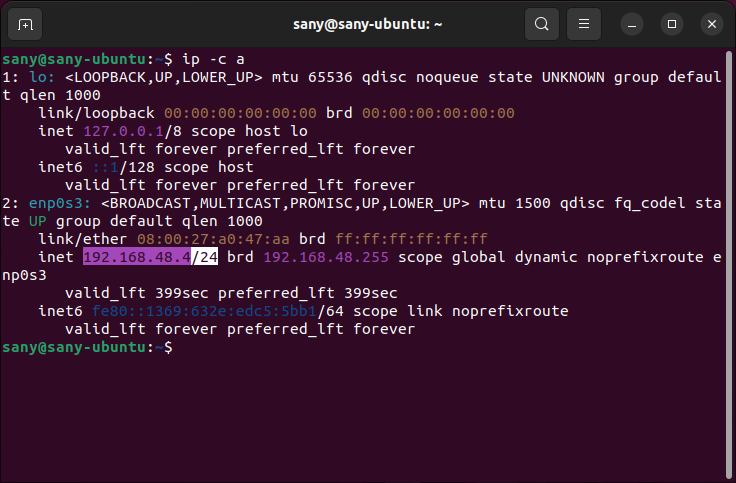
\includegraphics[width=0.5\textwidth]{images/ubuntu2.0_ip.PNG}
    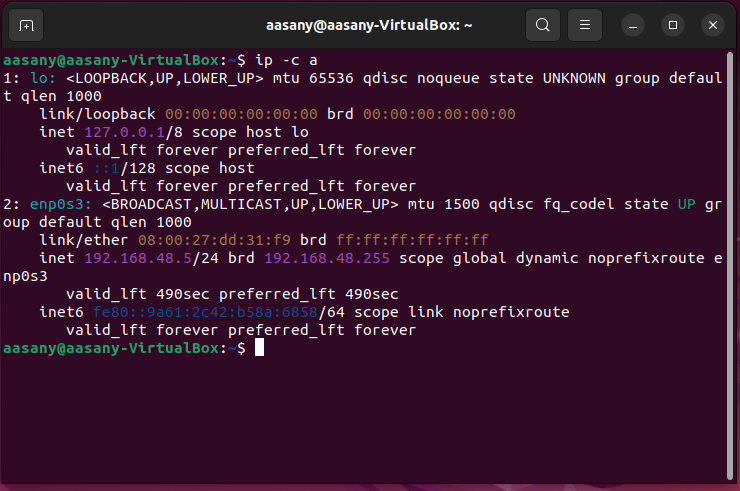
\includegraphics[width=0.5\textwidth]{images/ubuntu3.0_ip.PNG}\\\\
    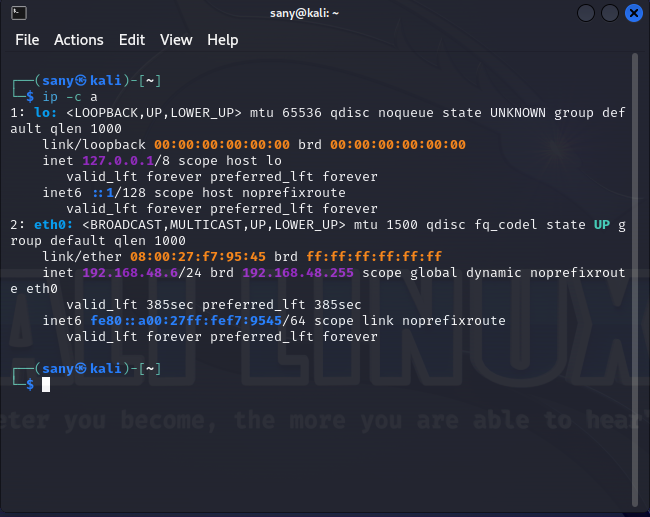
\includegraphics[width=0.5\textwidth]{images/kali_linux_ip.PNG}
    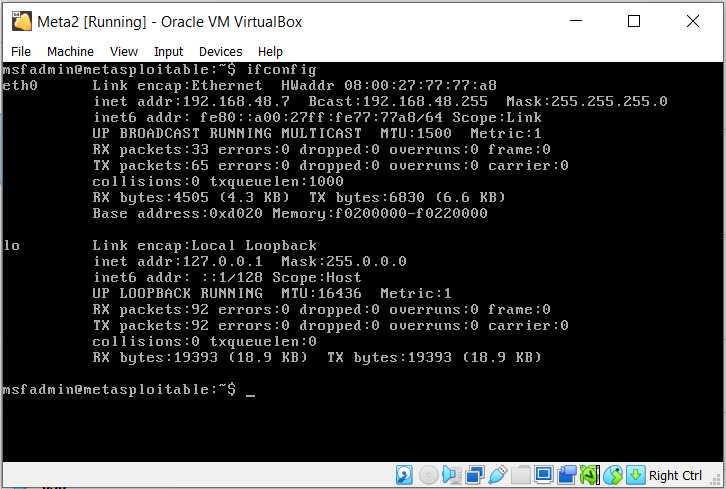
\includegraphics[width=0.5\textwidth , height=0.29\textheight]{images/meta2_ip.PNG}
\end{itemize}
\clearpage
\begin{itemize}
    \item \textbf{Threading and shared memory allow us to scale Snort3 to our network and create a much faster start-up.}
    \item \textbf{This allows multiple packet processing to free up more memory for more packet processing power.}\\\\
    So, we use snort3 instead of snort2. The version of our snort is:\\\\
    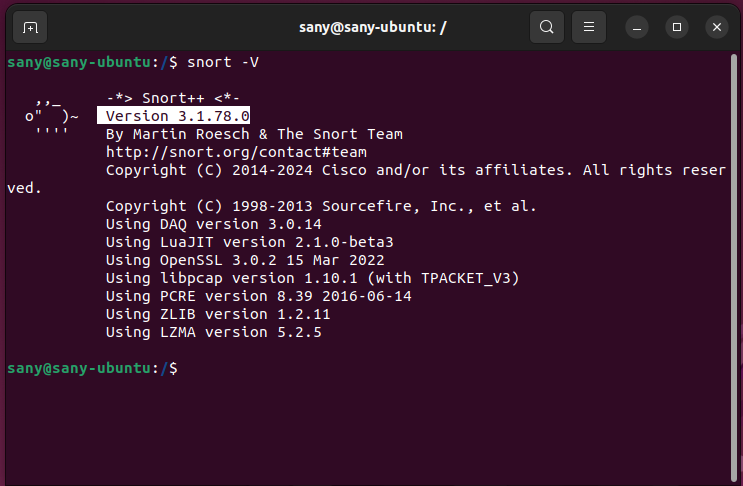
\includegraphics[width=1.0\textwidth]{images/snort_version.PNG}
\end{itemize}
\clearpage
\textbf{Snort3 Configuration}
\begin{itemize}
    \item Home NET:192.168.48.0/24
    \item EXTERNEL NET:!HOME NET\\\\
    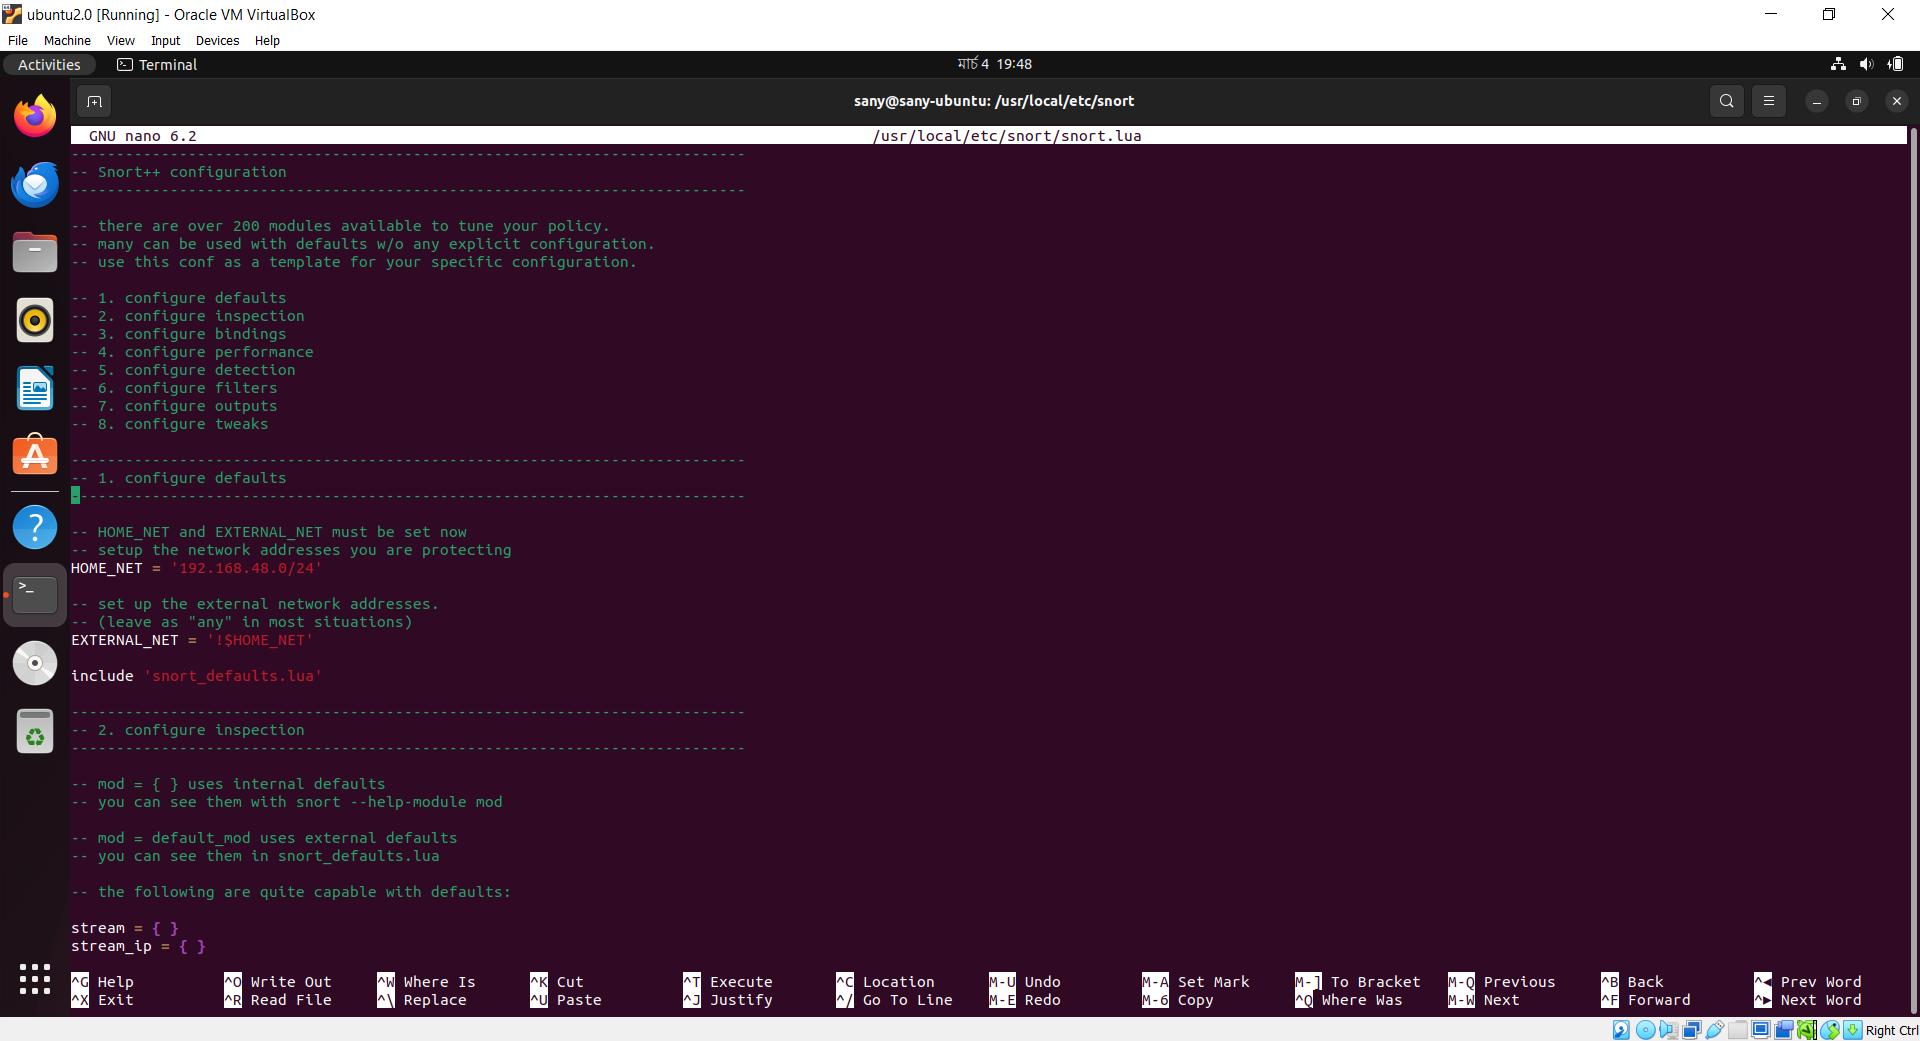
\includegraphics[width=1.0\textwidth]{images/configuration.PNG}\\\\
    \item \textbf{local.rules file created to write custom rules:}\\\\
    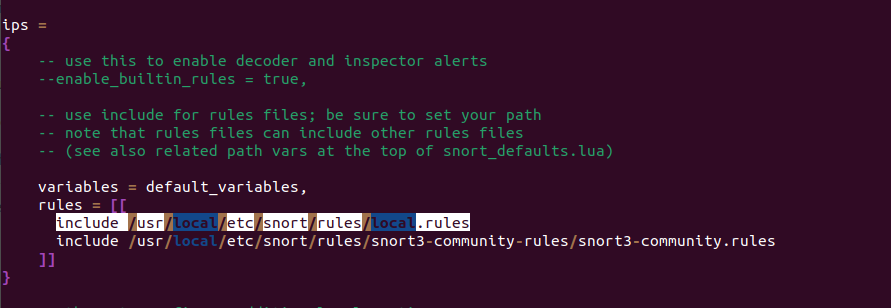
\includegraphics[width=1.0\textwidth]{images/local_rules_file.PNG}
\end{itemize}
\clearpage
\textbf{\hspace{-\3.5cm}Snort3 Community Rules}\\\\
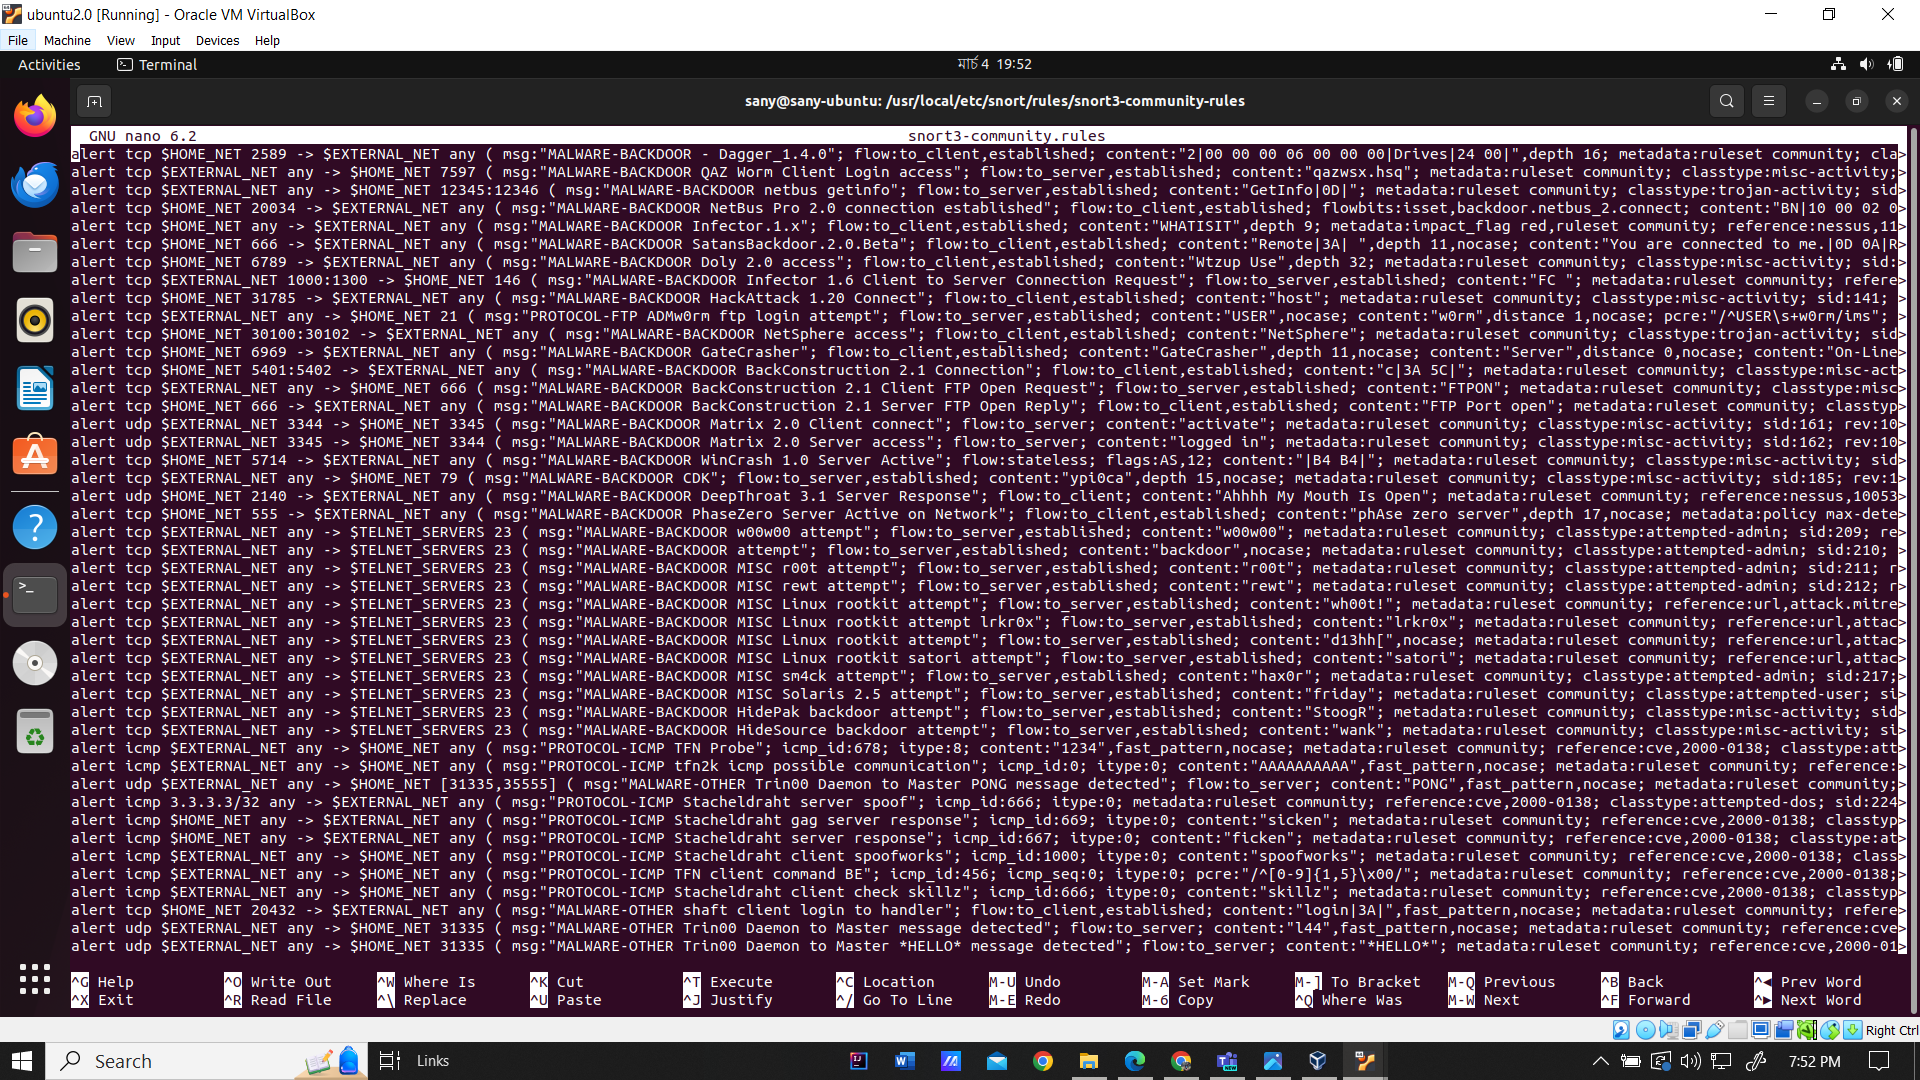
\includegraphics[width=1.0\textwidth]{images/community_rules.PNG}\\\\
\textbf{Snort3 Custom Rules}\\\\
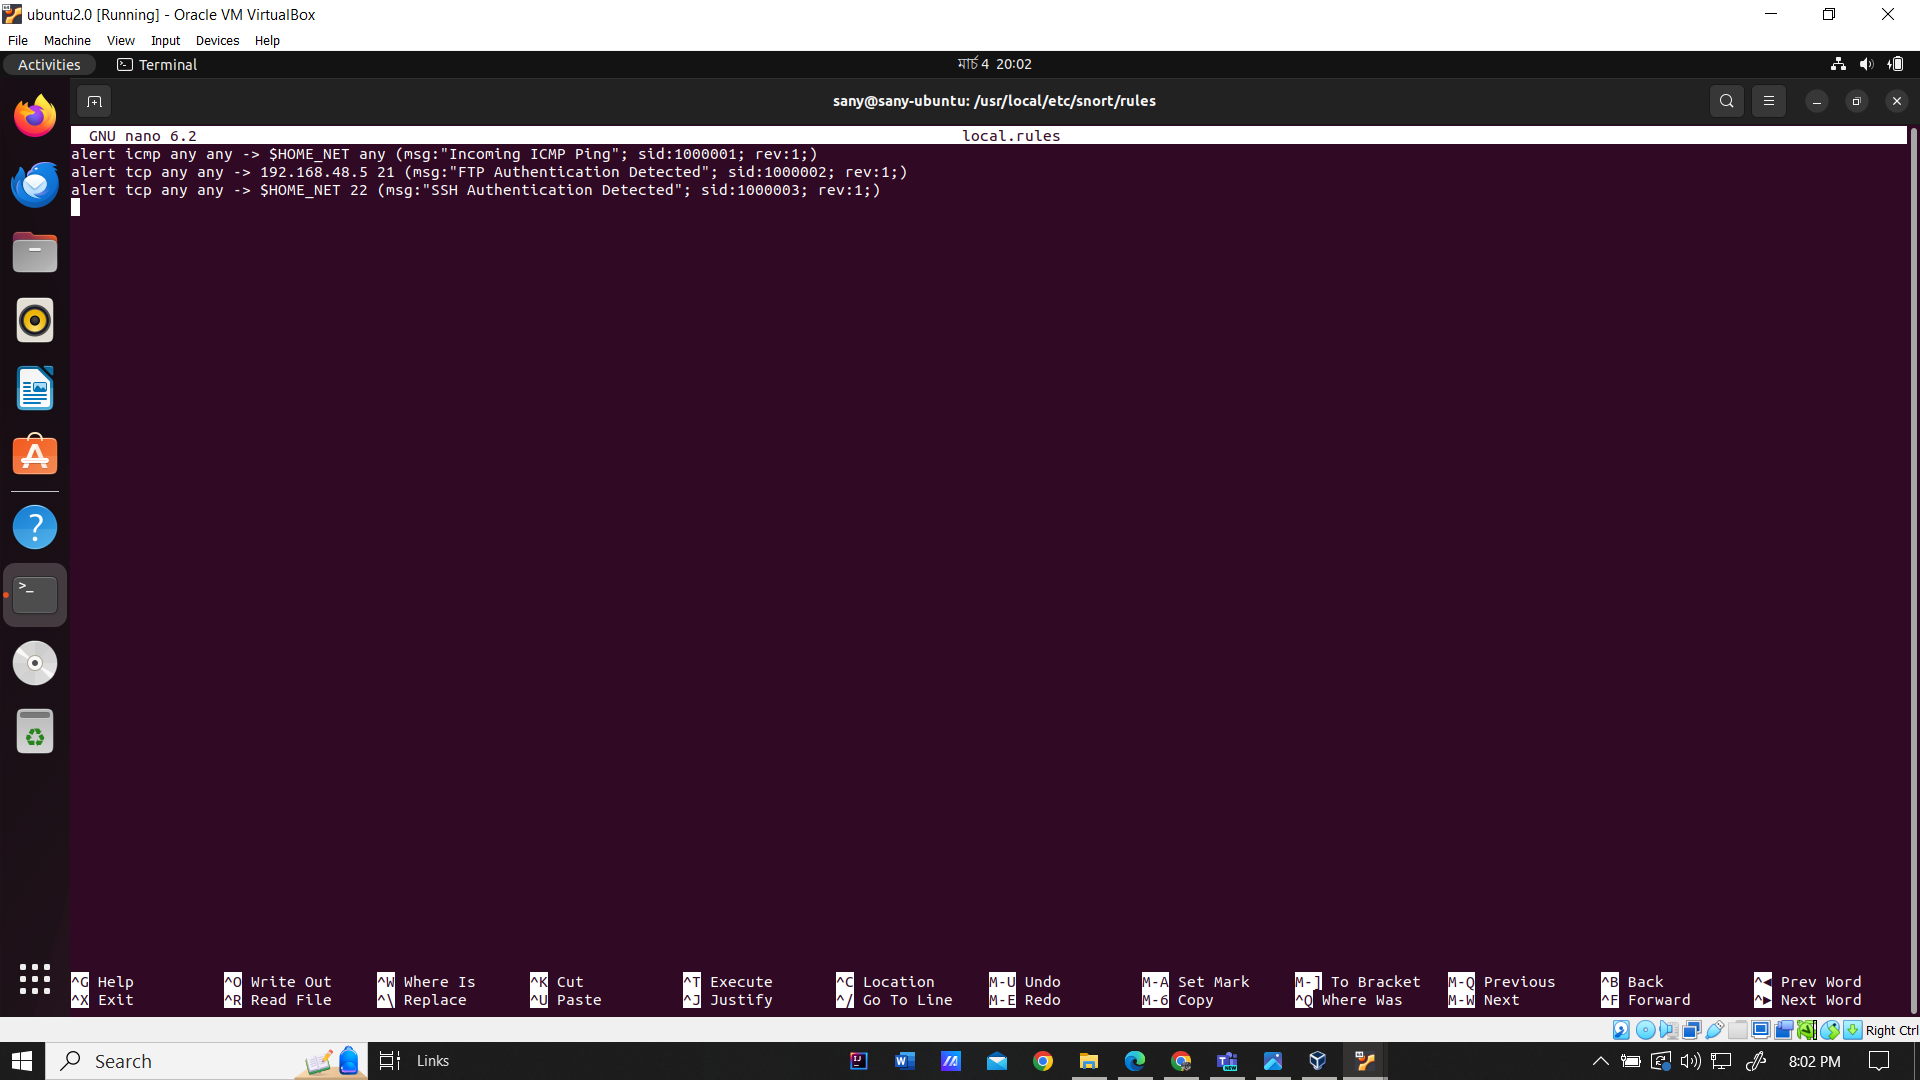
\includegraphics[width=1.0\textwidth]{images/custom_rules.PNG}
\clearpage
\textbf{\hspace{-\3.5cm}Custom rules explanation}\\\\
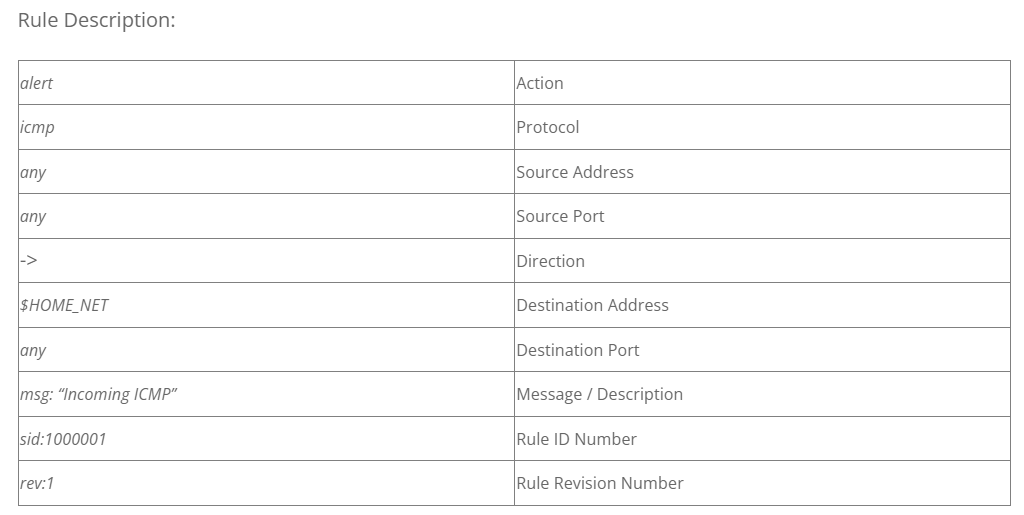
\includegraphics[width=1.0\textwidth]{images/custom_rules_desc.PNG}\\\\
\textbf{Snort3 manual trigger}\\\\
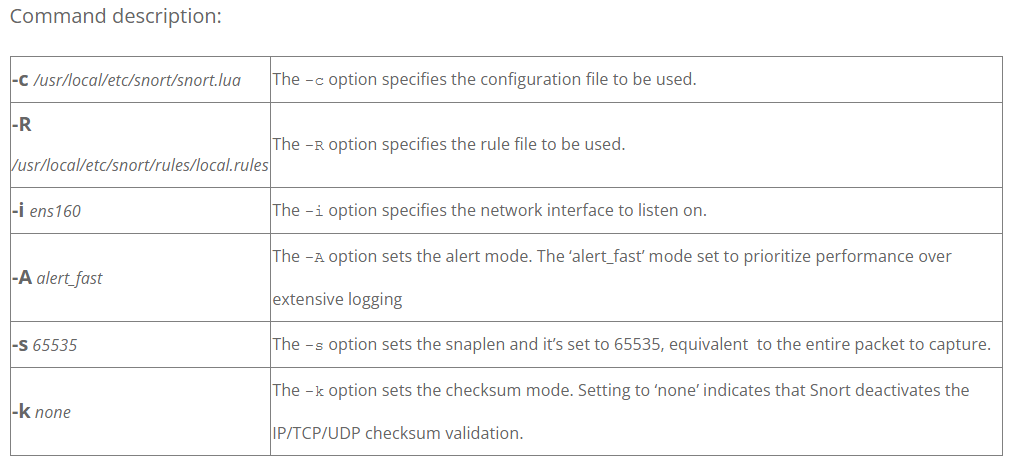
\includegraphics[width=1.0\textwidth]{images/manual_trig_3.PNG}\\\\
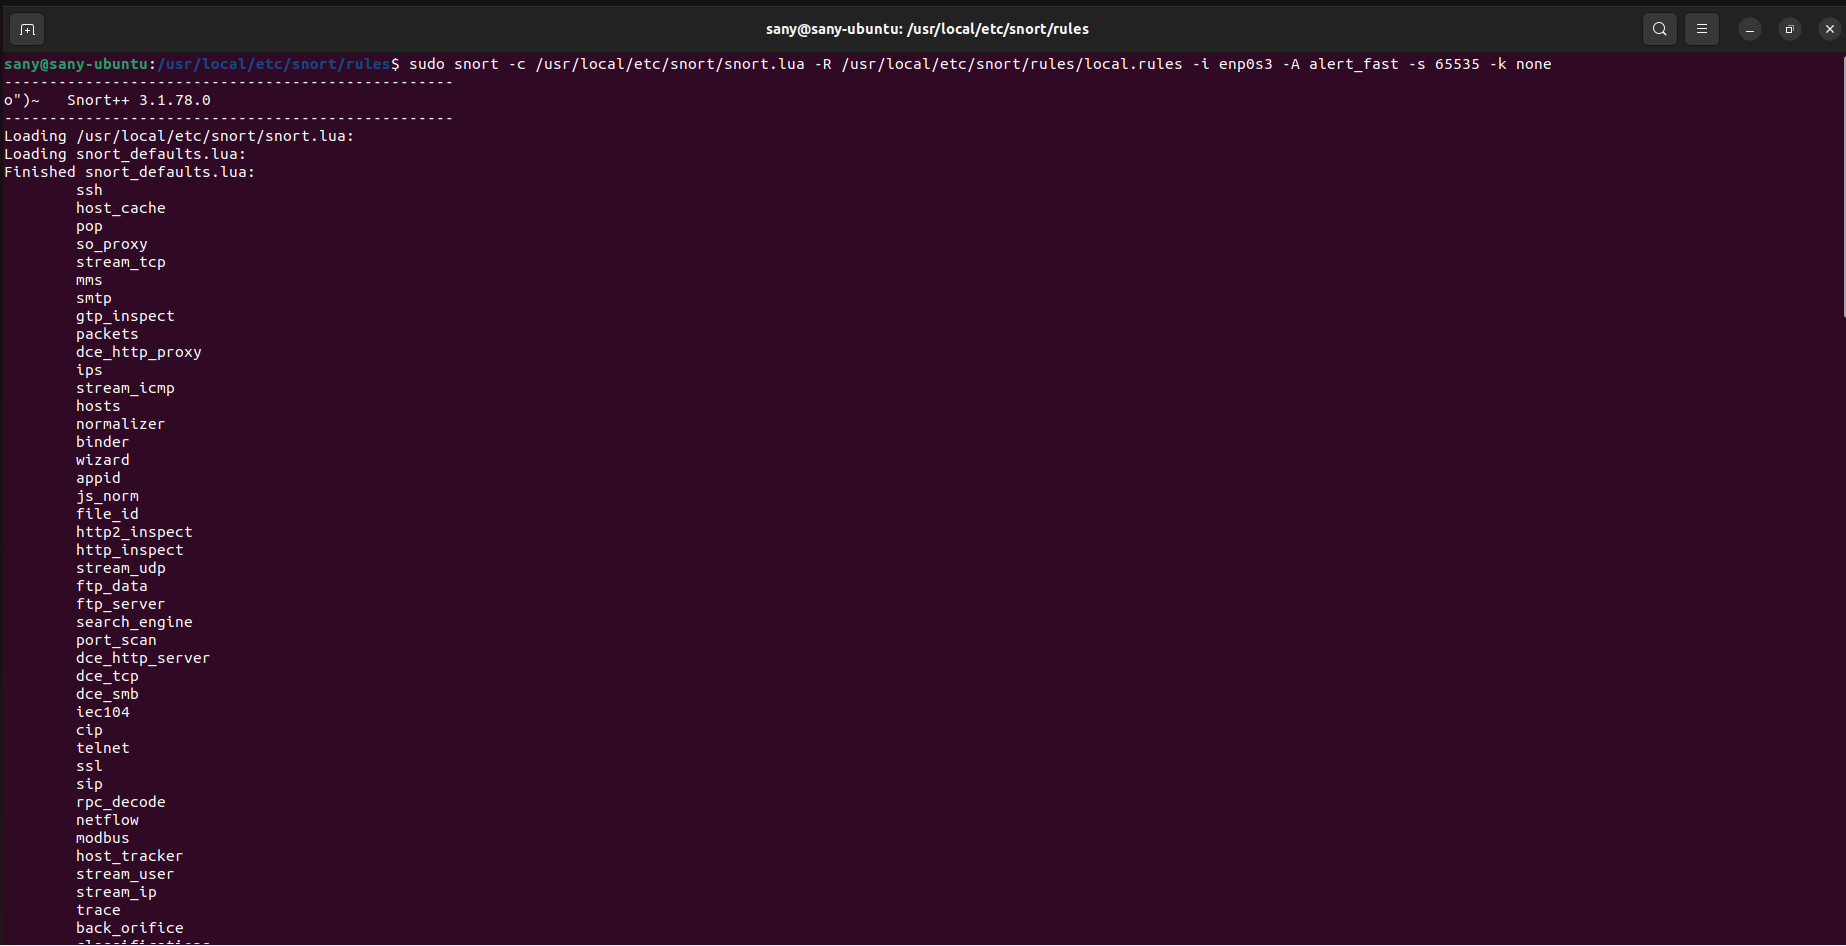
\includegraphics[width=1.0\textwidth]{images/manual_trig_1.PNG}
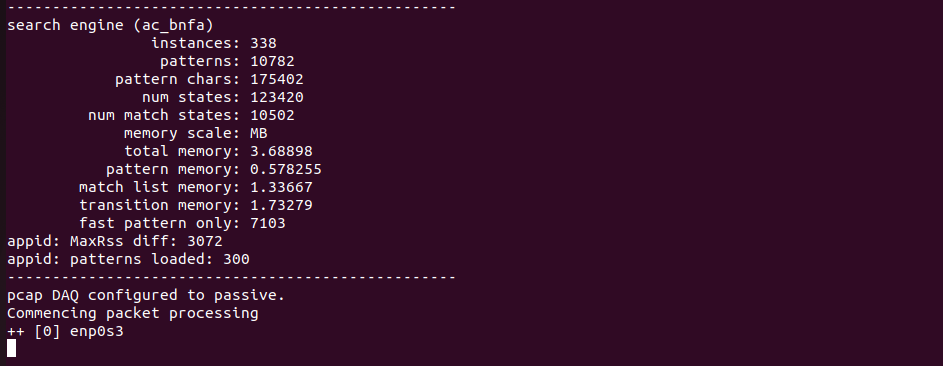
\includegraphics[width=1.0\textwidth]{images/manual_trig_2.PNG}\\\\
\clearpage
\textbf{A ping command is executed from Kali Linux to test the connectivity to our Ubuntu 2.0}\\\\
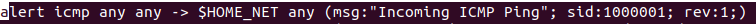
\includegraphics[width=1.0\textwidth]{images/ping1.PNG}
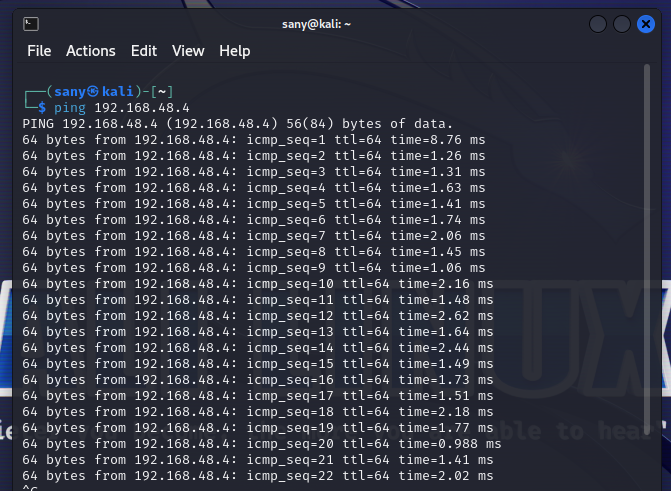
\includegraphics[width=1.0\textwidth,height=0.4\textheight]{images/ping2.PNG}
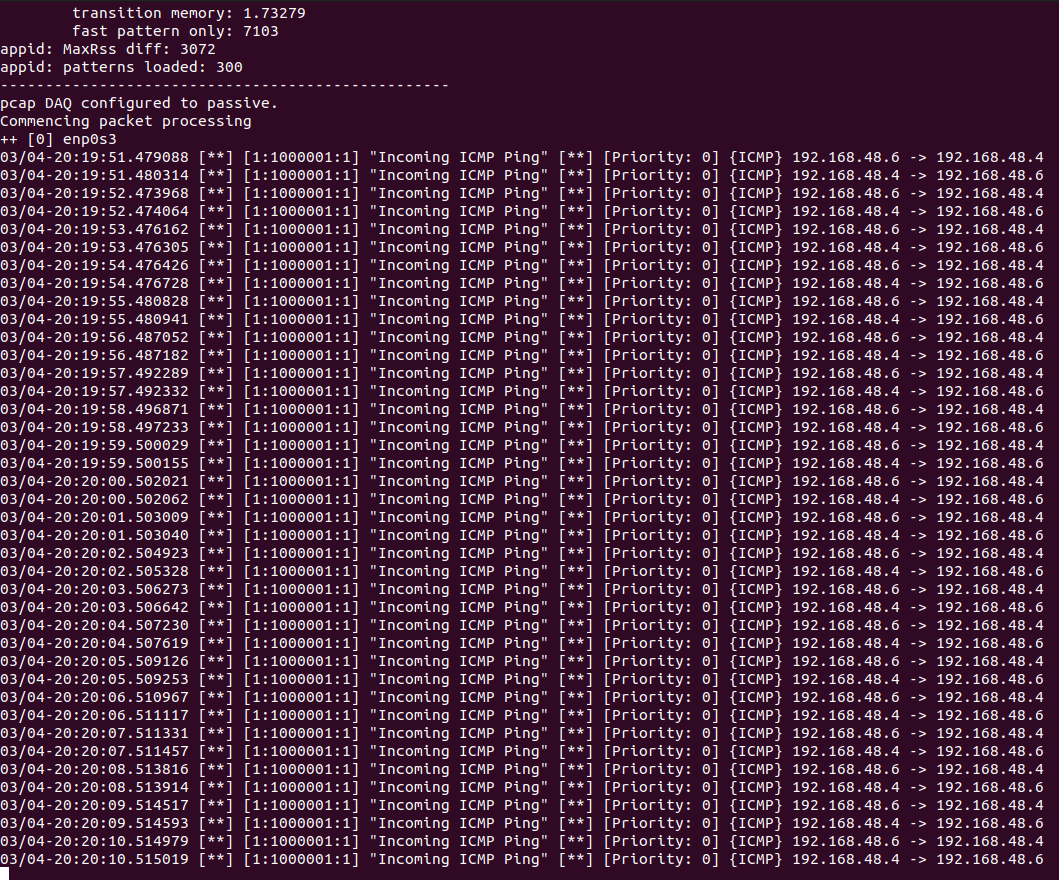
\includegraphics[width=1.0\textwidth,height=0.4\textheight]{images/ping3.PNG}
\clearpage
\textbf{To initiate an FTP (File Transfer Protocol) connection to Ubuntu 3.0 on port 21 from Kali Linux.}\\\\
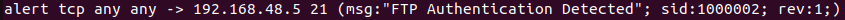
\includegraphics[width=1.0\textwidth]{images/ftp1.PNG}
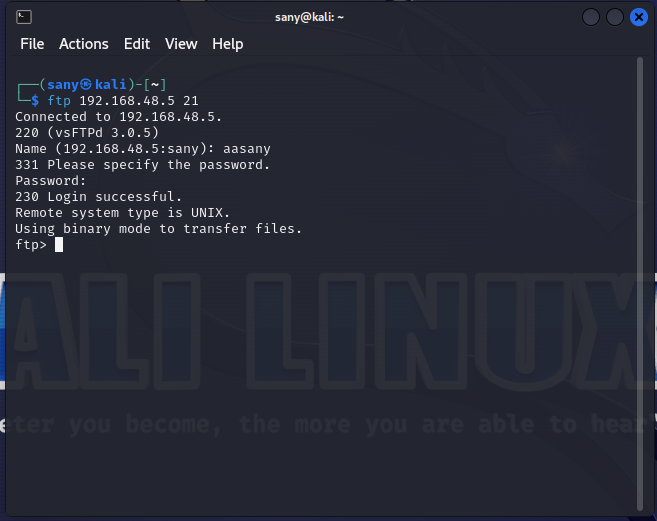
\includegraphics[width=1.0\textwidth,height=0.4\textheight]{images/ftp2.PNG}
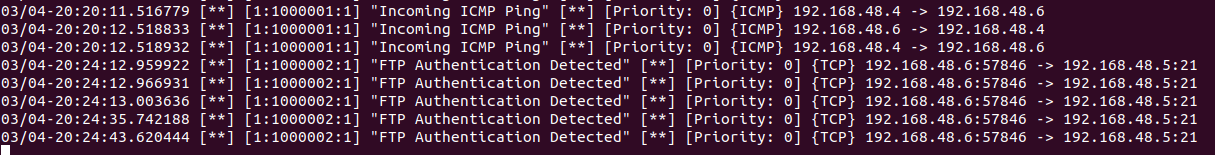
\includegraphics[width=1.0\textwidth]{images/ftp3.PNG}
\clearpage
\textbf{To establish an SSH connection to Metasploit2 with specific configuration options from Kali Linux.}\\\\
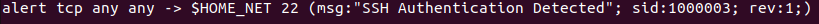
\includegraphics[width=1.0\textwidth]{images/ssh1.PNG}
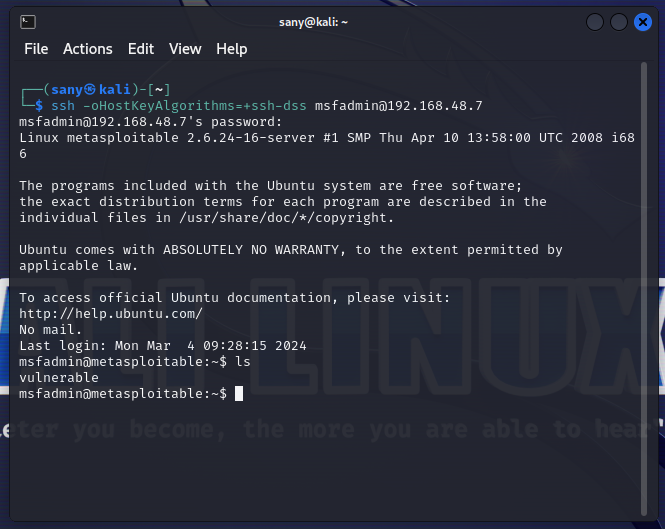
\includegraphics[width=1.0\textwidth,height=0.4\textheight]{images/ssh2.PNG}
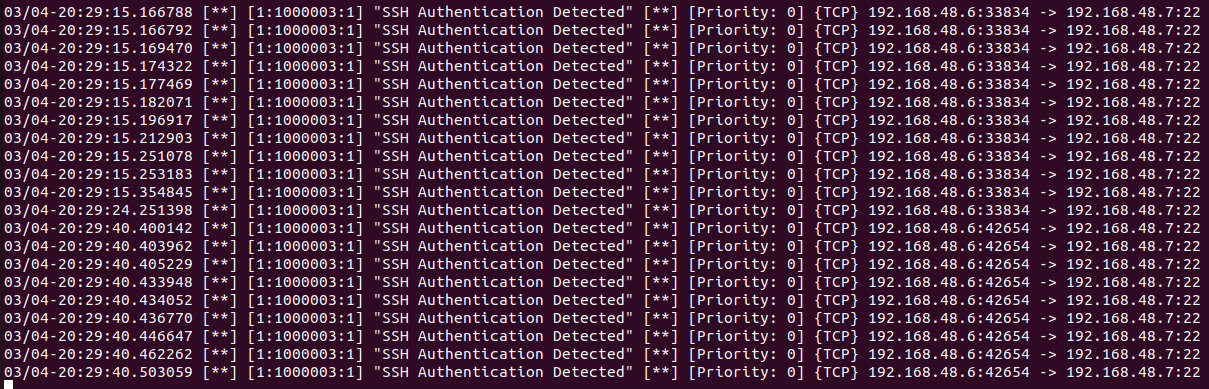
\includegraphics[width=1.0\textwidth,height=0.4\textheight]{images/ssh3.PNG}
\clearpage
\textbf{\hspace{-\3.5cm}Snort3 IDS Logging}\\
Packet logging in Snort refers to the process of capturing and recording network packets that match specific rules or signatures defined in the Snort intrusion detection system (IDS) configuration. Snort3 gives us the ability to log the intrusions in various file structure as we wish. For Snort to be an effective intrusion detection tool, it should log all alerts and store them on a local file or on a remote log server. Snort3 provides multiple options to log the Snort alerts. This latest update on Snort significantly improves the logging format that is compatible with the modern log management tools.\\\\
\textbf{Logging in JSON structure}\\\\
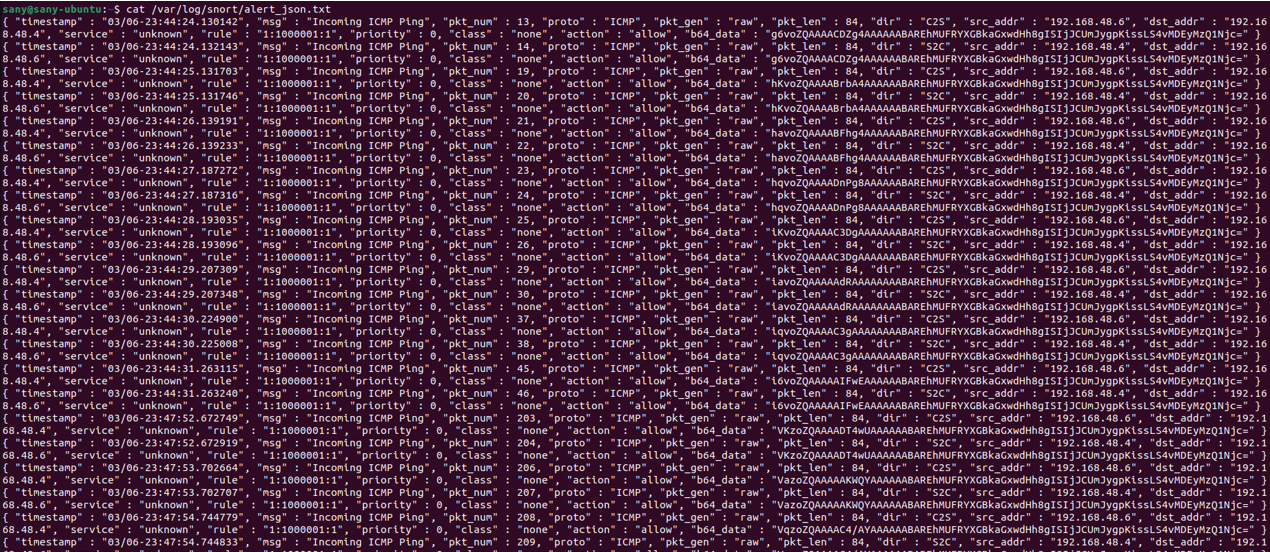
\includegraphics[width=1.0\textwidth]{images/json.PNG}
\clearpage
\textbf{\hspace{-\3.5cm}Logging in CSV structure}\\\\
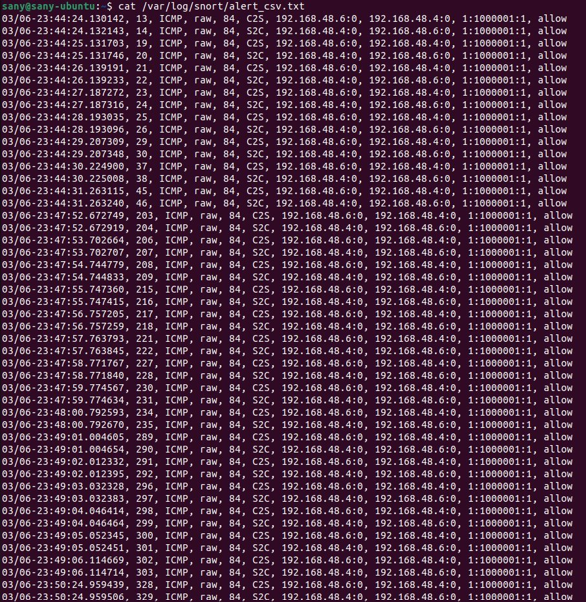
\includegraphics[width=1.0\textwidth]{images/csv.PNG}
\clearpage
\textbf{\hspace{-\3.5cm}A problem about where to set up snort:}\\\\
\textbf{\underline{Problem Statement}\\} 
If a subscriber configures Snort to operate as a sniffer, it will scan network packets and identify them. Snort can also log those packets to a disk file.To use Snort as a packet sniffer, users set the host's network interface to promiscuous mode to monitor all network traffic on the local network interface. But what happens when the packets are coming from outside the LAN?\\\\
\textbf{\underline{Solution}}\\
When packets are coming from outside the LAN (Local Area Network), such as from the internet or another external network, Snort can still capture and analyze them if it is deployed in a position where it can see the traffic.\\
Here's what happens:

\textbf{Placement:} Snort needs to be placed in a network segment where it can see the traffic. This could be at a network perimeter, where the LAN connects to the internet, or within a demilitarized zone (DMZ) if the network architecture includes one.

\textbf{Network Tap or Port Mirroring:} Snort can capture packets coming from outside the LAN by using network taps or by configuring port mirroring on network switches. Network taps directly copy the traffic passing through a network segment to a monitoring interface where Snort can capture it. Port mirroring, also known as SPAN (Switched Port Analyzer) or RSPAN (Remote SPAN), replicates traffic from one or more ports to another port where Snort is connected.

\textbf{Promiscuous Mode:} Snort's interface must still be set to promiscuous mode, regardless of whether the traffic is coming from inside or outside the LAN. This mode allows the network interface to capture all packets on the network segment, not just those intended for the host running Snort.

\textbf{Analysis:} Once Snort captures the packets, it can analyze them using its rulesets to detect any suspicious or malicious activity. This includes traffic originating from outside the LAN that may be attempting to exploit vulnerabilities or perform unauthorized activities.

In summary, while Snort is typically deployed within LANs to monitor internal traffic, it can also be configured to monitor and analyze traffic coming from outside the LAN by being placed strategically within the network architecture and using appropriate capture methods like network taps or port mirroring.
\clearpage
\section{Conclusion}
\label{sec:Conslusion}
 In conclusion, Snort is a powerful and versatile intrusion detection and prevention system that plays a crucial role in network security. It operates based on predefined rules and can analyze network traffic in real-time, making it effective in detecting and responding to a wide range of malicious activities. Whether used for packet logging, packet sniffing, network intrusion detection, or network intrusion prevention, Snort provides valuable insights into network traffic and helps organizations defend against evolving cyber threats. Its open-source nature and extensive community support make it a valuable tool in the arsenal of network security solutions, ensuring the continued resilience of modern network infrastructures.
\end{document}
